\chapter{Motion Tracking}
Just to introduce the topic, we can say that motion tracking is the process of determining the movement of an object in a video sequence. 
More in general, it regards the understanding of \textit{what} is moving in a scene and \textit{how} it moves/interacts with the environment.
This is a very important topic in computer vision, and it is used in many applications, such as video surveillance, traffic monitoring, human-computer interaction and biological applications (cell tracking). 
At high level, motion tracking can be used for the discovery of activities, behavior understanding, and detection of threats.
In this chapter, we will discuss the basic concepts of motion tracking, and we will present some of the most common algorithms used in this field.

\section{Object Tracking}
Object tracking is the process of locating a moving object over time. On the basis of the applications requirements, we can track the 2D coordinates (centroid), track in 3D (more cameras are required), or determine the position of complex objects (human body articulations).
The main goal of object tracking is to estimate the state of the object at each frame, and to predict its future position.
The applications of object tracking are numerous, and they include monitoring and surveillance, such as motion classification, identification of anomalous/suspicious behaviors, following a trajectory. 
Or again, human machine interfaces, such as interacting with a device removing physical barriers (mouse, keyboard), natural language understanding; or even virtual reality, such as immersive presence, animation of virtual characters.
Even mining and retrieval, such as browsing databases containing specific motion patterns.
\\
Some benefits of object tracking are:
\begin{itemize}
\item In HCI, control PC (or systems in general) à no need for additional tools;
\item In surveillance, Automated / Semi-automated systems à reduce the stress of human operators;
\item Virtual reality, computer animation à animate and drive the avatar;
\item But also: Training of athletes, Gait disorders detection, Medical applications, etc.
\end{itemize}

\section{2D Tracking}
Sometimes it is enough to track the object in 2D, for example when the object is moving on a plane.
Exists different approaches to 2D tracking:
\begin{itemize}
\item \textbf{Region-based} $\Rightarrow$ set of pixels that share similar features (color);
\item \textbf{Contour-based} $\Rightarrow$ determine position and shape of an object over time. Useful to track deformable objects;
\item \textbf{Feature-based} $\Rightarrow$ select meaningful points (contours, corners);
\item \textbf{Template-based} $\Rightarrow$ use specific models (hands, faces, eyes).
\end{itemize}

\subsection{Region-based tracking}
When it comes to real-time applications, tracking regions with uniform appearance offers several benefits. 
It enables swift processing, often exceeding 30 frames per second, while maintaining a commendable balance between quality and speed. 
The idea revolves around identifying areas in an image that exhibit consistent color characteristics. 
These regions are akin to patches of similar color projected onto the image plane, often achieved through segmentation techniques like background suppression.

One fundamental requirement for successful region tracking is ensuring that these regions possess distinguishable colors. 
However, this method faces challenges, particularly in scenarios with variable illumination. 
Changes in lighting conditions can destabilize the uniformity of color, complicating the tracking process. 
To mitigate this issue, various compensation techniques can be employed, such as utilizing the hue and saturation components of the HSV color space or normalizing the RGB values. 
While these techniques work reasonably well indoors, outdoor settings may present more difficulties due to unpredictable lighting changes.

In terms of what we aim to track, the possibilities are diverse. 
It could involve monitoring any moving object, distinguishing between skin and non-skin regions (useful for applications like hand and face tracking), identifying specific colored areas, and more. 
The approach typically involves techniques such as color thresholding for uniform regions or utilizing color histograms.

However, tracking regions with uniform appearance isn't without its challenges. 
Color variations over time due to changes in illumination or object posture pose significant hurdles. 
Additionally, models of tracked objects need continual updates to adapt to evolving conditions.

One conceivable approach to tackle these challenges involves breaking down the object into smaller regions. 
Each region is then associated with a color vector or histogram, representing the average color values within that region. 
During tracking, the color of each region is computed, and the similarity to a reference model is assessed. 
If the ratio between the reference and current values is close to 1, it indicates a good match.

Histograms serve as a valuable tool in this process. 
They provide a quantified representation of the color distribution within a region, enabling comparisons between reference and current models. 
Different similarity measures can be employed for evaluation, such as bin-by-bin comparison: \[\cup (O_i^t, O_i^r) \sum_{n=1}^{U} min \{O_{i,n}^r, O_{i,n}^t\} \]
or Sum of Squared Differences (SSD): \[SSD(O_i^t, O_i^r) = \sum_{n=1}^{U} (O_{i,n}^r - O_{i,n}^t)^2 \]
Careful consideration must be given to the number of bins used in the histograms, striking a balance between granularity and computational efficiency.

In summary, tracking regions with uniform appearance offers a promising avenue for real-time applications, but it requires robust techniques to address challenges such as variable illumination and color changes over time. 
Techniques involving region division and histogram analysis can help in achieving accurate and efficient tracking in such scenarios.
\\\textit{NB: Shadows can be a problem in region-based tracking because are source of noise $\Rightarrow$ false positive. A shadow does not correspond to the motion of a real object, but it is a change in the color of the object. 
More specifically it's a variation of the luminance while chrominance remains ideally unaltered. To solve this problem, and obtain a proper tracking, shadows should be removed before tracking using a suitable algorithm.}

\section{Blobs extraction} 
An object can be made up by several blobs (\textit{NB:one for the torso, one for head...}), where blobs are aggregations of connected pixels that share common features.
Talking about features, we can consider also position, so pixel with similar color but far from the object must be discarded.
The typical application is in combination with a background suppression.
\subsection{Target association}
This is a procedure common to all trackers, not only region-based. In general, it is worth noting that detection is not carried out on a frame-basis.
This could lead to a lot of false positives, and it is computationally expensive.  
The idea is that once detected, targets are followed on a proximity basis. 
So, for example, background subtraction informs about the presence of motion, histograms characterize each moving objects, and then, unless occlusion occur, the target in the next frame should be the closest blob.
\begin{figure}[h]
\centering
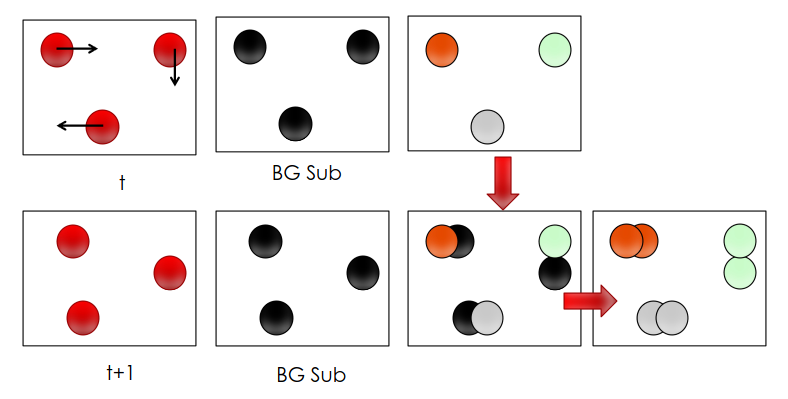
\includegraphics[width=0.7\textwidth]{Figures/Target_association.png}
\end{figure}

The steps of target association can be summed up as follows:
\begin{itemize}
\item Overlapping blob (issues with scale $\Rightarrow$ depends on objects size);
\item Centroid with minimum distance (as above);
\item Overlapping bounding boxes (may fail due to perspective);
\item Bounding box with minimum distance;
\item Bounding box to centroid distance.
\end{itemize}

\textit{NB: When association has been completed, for each object or blob update the appearance model to account for small variations. In presence of occlusions, the last saved model can be used to disambiguate.}

\subsection{Splitting}
The splitting is a common problem in blob extraction, and it is due to the fact that the object is composed by several blobs. If objects are identified as single blobs, there are no problems. However, background subtraction may return ambiguous results. 
Indeed, objects can be split into several small blobs, so this means that there is not enough separation between BG and FG. Or again, two objects can enter the scene together and then separate.
\begin{figure}[h]
    \centering
    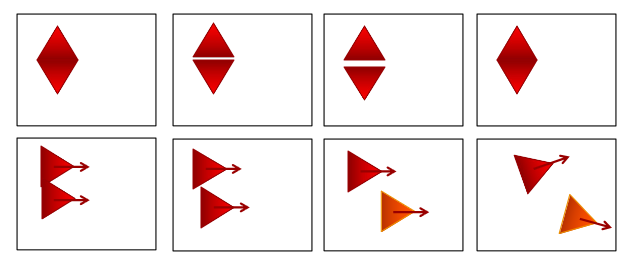
\includegraphics[width=0.7\textwidth]{Figures/Splitting.png}
\end{figure}

It is important to accumulate evidence before saying if it is case 1 or 2. It's impossible to understand what's going on immediately, so it is necessary a temporal interval to tell if the object merged even though it's fragmented or if it's two objects that are close to each other.

\section{Merging}
\begin{wrapfigure}{r}{0.4\textwidth}
    \centering
    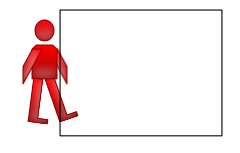
\includegraphics[width=0.25\textwidth]{Figures/Merging.png}
\end{wrapfigure}
Merging is the opposite of splitting, and it is due to the fact that two objects are identified as a single blob. This can happen when two objects are close to each other and move together consistently (then perhaps they're the same object).
An example can be when a person’s arm and foot enter the scene first and are detected as two well-separated FG blobs. 
Then also the rest of the body enters and a single blob is created. 

\subsection{Criteria for splitting and merging}
Observation is the key. We need to monitor the regions of interest and evaluate consistency in terms of:
\begin{itemize}
    \item Direction of motion;
    \item Distance between centroids/bounding boxes;
    \item Temporal range in which the phenomenon is observed;
    \item Velocity;
    \item Matching in features.
\end{itemize}

\section{Occlusion}
Occlusion is an anomalous, but very frequent, situation in tracking, and it occurs when moving objects overlap.
Consequently, one or more objects disappear from the scene and bigger blobs appear as a result of the occlusion, with properties that don't belong to any of the models acquired previously, so the acquisition models are not reliable anymore.\textit{NB: Model update should be avoided during occlusions.}
In order to solve this problem, we need to re-associate "A to A" and "B to B" (where A and B are the objects that are occluded). \textit{NB: Histograms are a good way out.}

\section{Tracking: Feature-based}
The objective is to retrieve the motion information of a set of features (such as points, corners, edges\dots) in the image.
\\Considering
\[A = \{A(0), A(1), A(2), \dots, A(j-1)\}\] as a set of images and
\[m_i(x_i, y_i)i = [0, j-1] \] the position of the feature in the image plane in each frame.
The objective is to determine the displacement vector \[d_i = (dx_i, dy_i)\] that best estimates the position of the feature in the next frame \[m_{i+1}(x_{i+1}, y_{i+1}) = m_i + d_i\]
If needed, points can be grouped and objects can be represented using the bounding box or the convex hull.
\\TODO: inserire immaginina maybe
\\The question now is how to choose a good feature point that must has distinctive characteristic such as brightness, contrast, texture, edges, corners or point with high curvature.
\\The main idea is that for each candidate point, we compute: 
\\TODO: inserisci matrice
\\Where $J_x$ and $J_y$ are the gradients evaluated on the point in $x$ and $y$ direction within $W$ ($nxn$ window). 
A good feature point is the one that maximizes the function, so the point where the smallest eigenvalue of $Z$ is larger than a specific threshold.
In practice, it highlights corner points and texture.
\\To sum up a little bit the important things:
\begin{itemize}
    \item Eigenvalues should be above the image noise;
    \item Small eigenvalues imply strong similarity within the window;
    \item A large and a small eigenvalue means unidirectional patterns;
    \item If both eigenvalues are large, the point is of high interest (salt\&pepper texture, corners).
\end{itemize}

For what concerns tracking them, we must ensure that the same points are tracked throughout the video sequence. 
Ideally we would expect that $A_i(Dm-d)=A_{i+1}(m)$, where $A_i, A_{i+1}$ are the successive frames at time $i$ and $i+1$, $m$ is the 2D position of the feature point, $D$ the deformation matrix (affine transformation model) and $d$ is the displacement vector (translation models).
\\ However, due to noise the equality usually does not hold. In addition, motion across successive frames is assumed to be small $\Rightarrow$ a translational model is a good approximation.
Feature dissimilarity measure is used to quantify the change of appearance between the first and current frame
\[
    \varepsilon = \iint_{W} \left(A_i(m-d)-A_{i+1}(m)\right)^2 w(m) \, dm
\]
where $w$ is a weighting function such as Gaussian to emphasize the center of the window\dots
\\When the feature dissimilarity grows too large, the feature point should be abandoned and a new one should be selected.
To minimize the residual we differentiate w.r.t unknowns (d)
\[
    e = 2 \iint_{W} \left(A_i(m)-A_{i+1}(m)\right)g(m) \, w(m) \, dm
\] 
and 
\[
    g(m)=\begin{bmatrix}
        \frac{\partial (A_i(m)-A_{i+1}(m))}{\partial x} \\
        \\
        \frac{\partial (A_i(m)-A_{i+1}(m))}{\partial y} 
    \end{bmatrix}
\]
In this case the solution for the displacement vector can be expressed by the 2x2 linear system of equations $Zd = e$.
\subsection{The Lucas-Kanade optical flow}
Substantially is a two-frame differential method for optical flow estimation.
Consider $u=\left[u_x, u_y\right]$ in frame $I$ and $v=\left[v_x, v_y\right]$ in frame $J$ the goal is to find $d$ that satisfies the equation $v = u + d$ such as $I$ and $J$ are similar(translation model).
Because of the aperture problem, similarity must be defined in 2D.
$d$ is the vector that minimizes
\[
    \varepsilon(d) = \epsilon(d_x, d_y) = \sum_{x=u_x-w_x}^{u_x+w_x} \sum_{y=u_y-w_y}^{u_y+w_y} \left[I(x, y) - J(x+d_x, y+d_y)\right]^2
\]
\\TODO:Da qui in poi è letteralmente copia incolla delle slide\\
We use an integration window to compute the displacement vector. 

\subsection{Pyramidal implementation}
The two key components to any feature tracker are accuracy and robustness.
Accuracy relates to the local sub-pixel accuracy attached to tracking $\Rightarrow$ small integration window preferable to limit
smoothness and preserve detail information (two image
patches moving rapidly in different directions).
Robustness relates to the sensitivity of tracking with respect to changes of light and big motions $\Rightarrow$ a large window is preferable.
$\Rightarrow$ Pyramidal implementation  *disegnino*
Level 0 is the image at original resolution.
Level 4, in the example, is the image at lowest resolution.
The L-th level is defined as a linear combination of the elements in the previous level.
\\ Conti da fare 

At each level of the pyramid an initial guess g of the flow is
computed at the lower level, which is then refined at the current
level.

g is used to pre-translate the image patch in the second image J
d should be small
the information is then propagated at the upper level

overall the displacement becomes


\subsection{Bayesian tracking}
The basic idea is to estimate the state of a system over discrete time steps.
At each step, we compute noisy measurements of the state and use them to update our estimate.
The state of the system is represented by the x-y coordinates, velocity and acceleration along each dimension(6D vector).
Important thing is that noise is typically smaller than the information about the state.
The state can be defined as \[x_k = f_k(x_{k-1} + w_{k-1})\]
Linking the measurement with the state vector we have \[z_k = h_k x_k + v_k\]
where $w_k$ is the process noise, $v_k$ is the measurement noise, $f_k$ and $z_k$ are in general nonlinear functions defined in the state space.
System and measurement should be available in probabilistic form.
Every time the measurement is available, the estimation can be computed.
It is an online method $\Rightarrow$ for every step k an estimate can be computed based on the
previous observations $z_k$ up to instant $k$.
The initial probability distribution of the state vector is given $\Rightarrow$ $p(x_0|z_0)$.
$z_0$ contains no measurement information, so it is the prior distribution.
The goal is to compute the posterior distribution $p(x_k|z_k)$ at time $k$.
The process consists of two steps:
\begin{itemize}
    \item Prediction: $p(x_k|z_{k-1})$ is computed;
    \item Update: $p(x_k|z_k)$ is computed.
\end{itemize}
Let's consider the prediction step\dots\\
From the previous representation we have \[p(x_k|z_{k-1}) = \int p(x_k|x_{k-1})p(x_{k-1}|z_{k-1})dx_{k-1}\]
This means that the posterior distribution at time $k-1$ is used to compute the prior distribution at time $k$, so it is propagated forward in time using the system model.
\\Using the Bayes theorem, it is possible to obtain the desired distribution \[p(x_k|z_k) = \frac{p(z_k|x_k)p(x_k|z_{k-1})}{p(z_k|z_{k-1})}\]
where $p(z_k|x_k)$ is the likelihood function, $p(x_k|z_{k-1})$ is the prior distribution and $p(z_k|z_{k-1})$ is the evidence and is used for normalization and computed as \[p(z_k|z_{k-1}) = \int p(z_k|x_k)p(x_k|z_{k-1})dx_k\]
\subsection{Bayesian traking- toy example}
TODO- tutto
\\section{Kalman filter}
The Kalman filter is a recursive algorithm that estimates the state of a linear dynamic system from a series of noisy measurements.
In a nutshell we can say the following things:
\begin{itemize}
    \item It is in line with the Bayesian tracking;
    \item It take a measurement;
    \item The measurement is subject to error;
    \item Derive the state of the system from the measurement.
\end{itemize}
We start from 